\subsection{Recurrent Neural Networks (RNN)}
A recurrent neural network (RNN) is a neural network that is specialized in processing a temporal sequence of data $x_1, \cdots,x_T$.

The term "recurrent" in their name refers to the execution of the same operations on each element $x_t$ of the sequence performed by this type of network, applying the same matrix of weights $V$.

This causes each output $o_t$ to depend on the previous ones, and for the network to maintain a hidden state $h_t$ directly dependent on the previous one $h_{t-1}$.

The image \vref{fig:recurrent_neural_network_unfold} shows an RNN unfolding over time (on the sequence) in a complete network.

\begin{figure}
	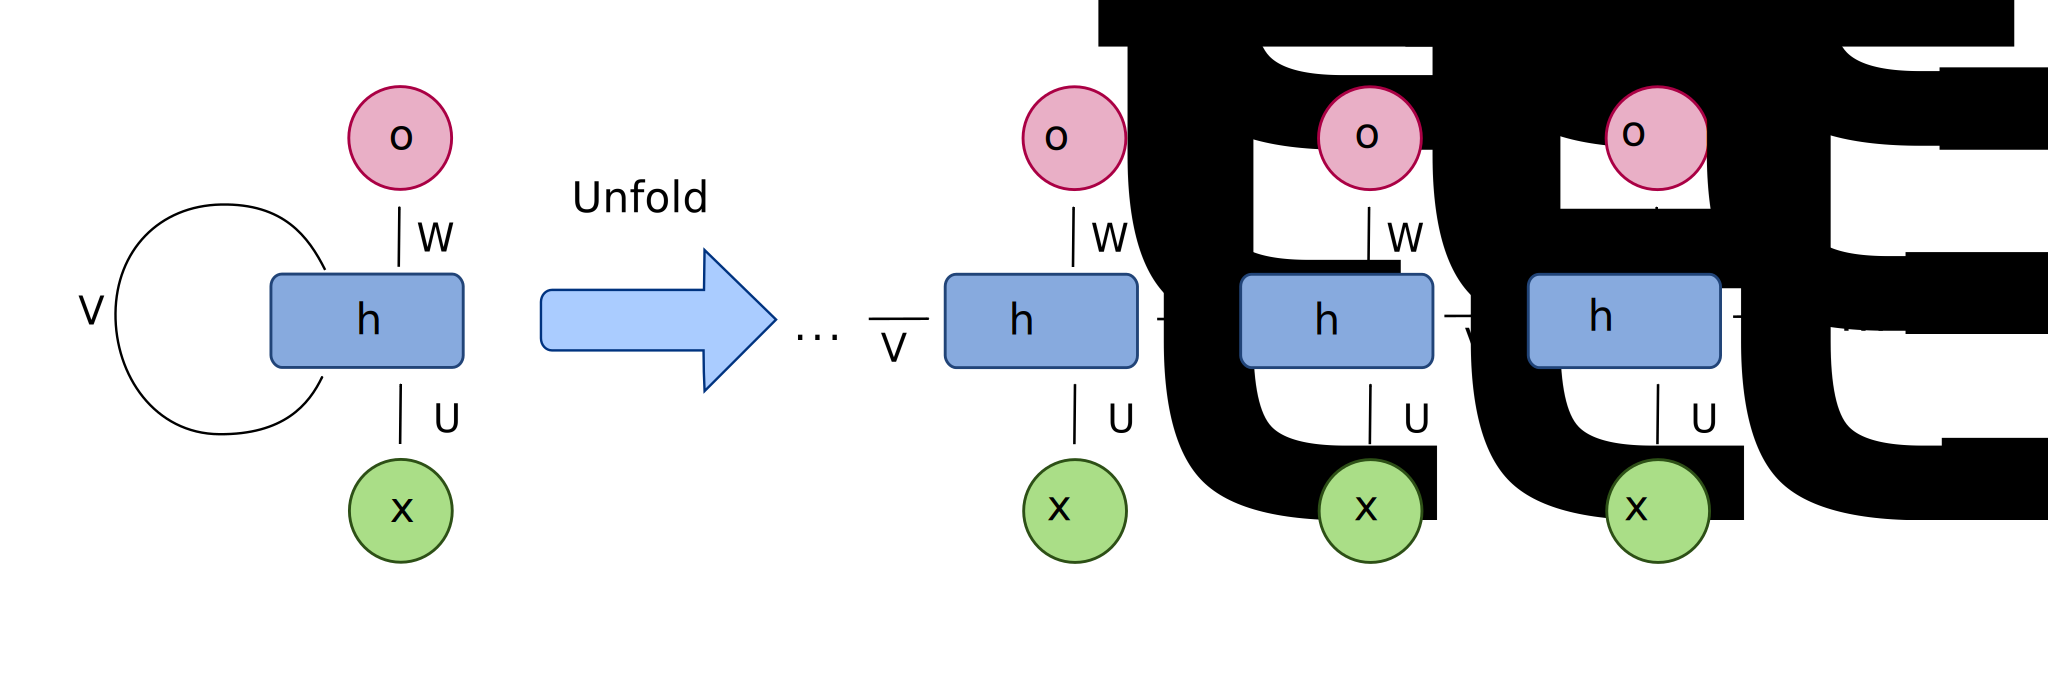
\includegraphics[width=0.5\textwidth]{images/recurrent_neural_network_unfold}
	\caption{Unrolling of a basic recurrent neural network, compressed on the left and unfolded on the right, source~\cite{wiki:rnn}.}
	\label{fig:recurrent_neural_network_unfold}
\end{figure}

We are going to analyze each element of the architecture of an RNN, explaining step by step how the information is processed within this type of network:
\begin{description}
	\item[input]: $x_t$ represents the input of the network at instant $t$;
	\item[hidden state]: $h_t$ represents the hidden state at time $t$, which acts as the "memory" of the network, being computed based on $x_t$ and the previous state $h_{t-1}$ by applying weight matrices, and an activation function $f$ (any nonlinear transformation such as $\tanh$, ReLU, $\dots$) and adding a bias vector $c$:
	$$
	h_{t}=f\left(U \cdot x_{t}+V \cdot h_{t-1}+c\right)
	$$
	\item[weights]: the connections between neurons of input-to-hidden type ($x_t$ to $h_t$) are parameterized by a matrix of weights $U$, while those of hidden-to-hidden type ($h_{t-1}$ to $h_t$) and hidden-to-output type ($h_t$ to $o_t$) are respectively parameterized by two weight matrices $V$ and $W$;
	\item[output]: $o_t$ represents the output of the network, which is also often subject to a nonlinear activation function $g$, especially when the network contains other layers.
	$$
	o_{t}=g\left(b_{t}+W \cdot h_{t}\right)
	$$ 
	where $b_{t}$ is the bias vector at time $t$
\end{description}
